% ----------------------------------------------------------------- %
%             The Speech Signal Processing Toolkit (SPTK)           %
%             developed by SPTK Working Group                       %
%             http://sp-tk.sourceforge.net/                         %
% ----------------------------------------------------------------- %
%                                                                   %
%  Copyright (c) 1984-2007  Tokyo Institute of Technology           %
%                           Interdisciplinary Graduate School of    %
%                           Science and Engineering                 %
%                                                                   %
%                1996-2017  Nagoya Institute of Technology          %
%                           Department of Computer Science          %
%                                                                   %
% All rights reserved.                                              %
%                                                                   %
% Redistribution and use in source and binary forms, with or        %
% without modification, are permitted provided that the following   %
% conditions are met:                                               %
%                                                                   %
% - Redistributions of source code must retain the above copyright  %
%   notice, this list of conditions and the following disclaimer.   %
% - Redistributions in binary form must reproduce the above         %
%   copyright notice, this list of conditions and the following     %
%   disclaimer in the documentation and/or other materials provided %
%   with the distribution.                                          %
% - Neither the name of the SPTK working group nor the names of its %
%   contributors may be used to endorse or promote products derived %
%   from this software without specific prior written permission.   %
%                                                                   %
% THIS SOFTWARE IS PROVIDED BY THE COPYRIGHT HOLDERS AND            %
% CONTRIBUTORS "AS IS" AND ANY EXPRESS OR IMPLIED WARRANTIES,       %
% INCLUDING, BUT NOT LIMITED TO, THE IMPLIED WARRANTIES OF          %
% MERCHANTABILITY AND FITNESS FOR A PARTICULAR PURPOSE ARE          %
% DISCLAIMED. IN NO EVENT SHALL THE COPYRIGHT OWNER OR CONTRIBUTORS %
% BE LIABLE FOR ANY DIRECT, INDIRECT, INCIDENTAL, SPECIAL,          %
% EXEMPLARY, OR CONSEQUENTIAL DAMAGES (INCLUDING, BUT NOT LIMITED   %
% TO, PROCUREMENT OF SUBSTITUTE GOODS OR SERVICES; LOSS OF USE,     %
% DATA, OR PROFITS; OR BUSINESS INTERRUPTION) HOWEVER CAUSED AND ON %
% ANY THEORY OF LIABILITY, WHETHER IN CONTRACT, STRICT LIABILITY,   %
% OR TORT (INCLUDING NEGLIGENCE OR OTHERWISE) ARISING IN ANY WAY    %
% OUT OF THE USE OF THIS SOFTWARE, EVEN IF ADVISED OF THE           %
% POSSIBILITY OF SUCH DAMAGE.                                       %
% ----------------------------------------------------------------- %
\hypertarget{c2sp}{}
\name{c2sp}{transform cepstrum to spectrum}
{speech parameter transformation}

\begin{synopsis}
\item[c2sp] [ --m $M$ ] [ --l $L$ ] [ --p ] [ --o $O$ ] [ {\em infile} ]
\end{synopsis}

\begin{qsection}{DESCRIPTION}
{\em c2sp} calculates the spectrum from the minimum phase cepstrum 
from {\em infile} (or standard input), 
sending the result to standard output.
Input and output data are in float format.
\end{qsection}

\begin{options}
	\argm{m}{M}{order of cepstrum}{25}
	\argm{l}{L}{frame length}{256}
	\argm{p}{}{output phase}{FALSE}
	\argm{o}{O}{output format\\
                if the ``--p'' option is not assigned then
                \\
		\begin{tabular}{ll} \\[-1ex]
			$O=0$ & $20 \times \log |H(z)|$ \\
			$O=1$ & $\ln |H(z)|$ \\
			$O=2$ & $|H(z)|$ \\[1ex]
		\end{tabular}\\
		if the ``--p'' option is assigned then
		\\
		\begin{tabular}{ll}\\[-1ex]
			$O=0$ & $\arg |H(z)| \div \pi \quad [\pi \; rad.]$ \\
			$O=1$ & $\arg |H(z)| \quad [rad.]$ \\
			$O=2$ & $\arg |H(z)| \times180\div\pi\quad[deg.]$ \\
		\end{tabular}\\\hspace*{\fill}}{0}
\end{options}

\begin{qsection}{EXAMPLE}
The example below takes the 15-th order cepstrum from the file
 {\em data.cep} in float format, evaluates the running spectrum,
 and presents it in the screen:
\begin{quote}
 \verb! c2sp -m 15 data.cep | grlogsp -x 5 | xgr ! 
\end{quote}
\begin{center}
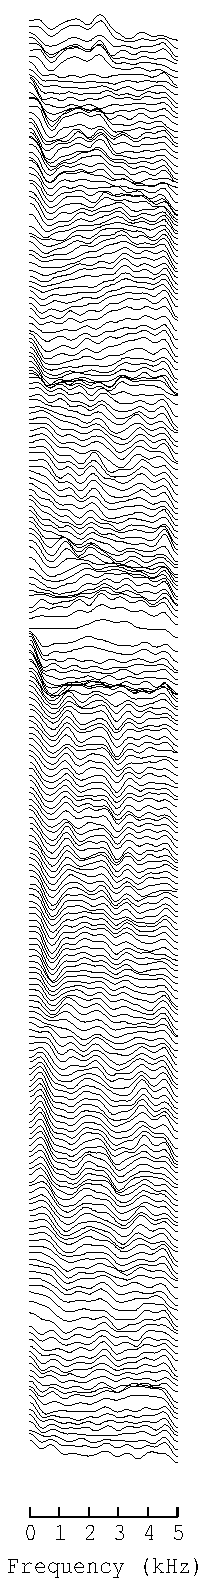
\includegraphics[width=3cm]{fig/c2sp.pdf}
\end{center}
\end{qsection}

\begin{qsection}{SEE ALSO}
\hyperlink{uels}{uels},
\hyperlink{mgc2sp}{mgc2sp}
\end{qsection}
